% file: 3-10-traversability/fleury-bridge.tex

\documentclass[tikz]{standalone}
\usetikzlibrary{positioning, fit, shapes}

\begin{document}
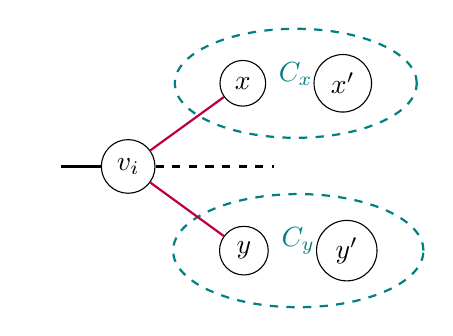
\begin{tikzpicture}[v/.style = {draw, circle, minimum size = 12pt},
    e/.style = {thick},
    node distance = 0.6cm and 1.0cm,
    comp/.style = {draw, thick, teal, dashed, ellipse, minimum width = 15pt}]

    \node (vi) [v] {$v_i$};
    \node (l) [v, draw = none, left = 0.50cm of vi] {};
    \draw [e] (l) to (vi);

    \node (x) [v, above right = of vi] {$x$};
    \node (x') [v, right = 0.60cm of x] {$x'$};
    \node (z) [v, draw = none, right = 1.50cm of vi] {};
    \draw [e, dashed] (vi) to (z);
    \node (y) [v, below right = of vi] {$y$};
    \node (y') [v, right = 0.60cm of y] {$y'$};

    \node (xcomp) [comp, fit = (x) (x')] {$C_{x}$};
    \node (ycomp) [comp, fit = (y) (y')] {$C_{y}$};
    % \node (zcomp) [comp, fit = (z), rotate fit = 90] {};

    \path (vi) edge[e, purple] (x)
	       edge[e, purple] (y);
\end{tikzpicture}
\end{document}
